\documentclass[tikz]{standalone}

\usepackage[latin1]{inputenc}
\usepackage{tikz}
\usetikzlibrary{shapes,arrows,calc,positioning,decorations.pathmorphing}
% GNUPL
\begin{document}
\pagestyle{empty}


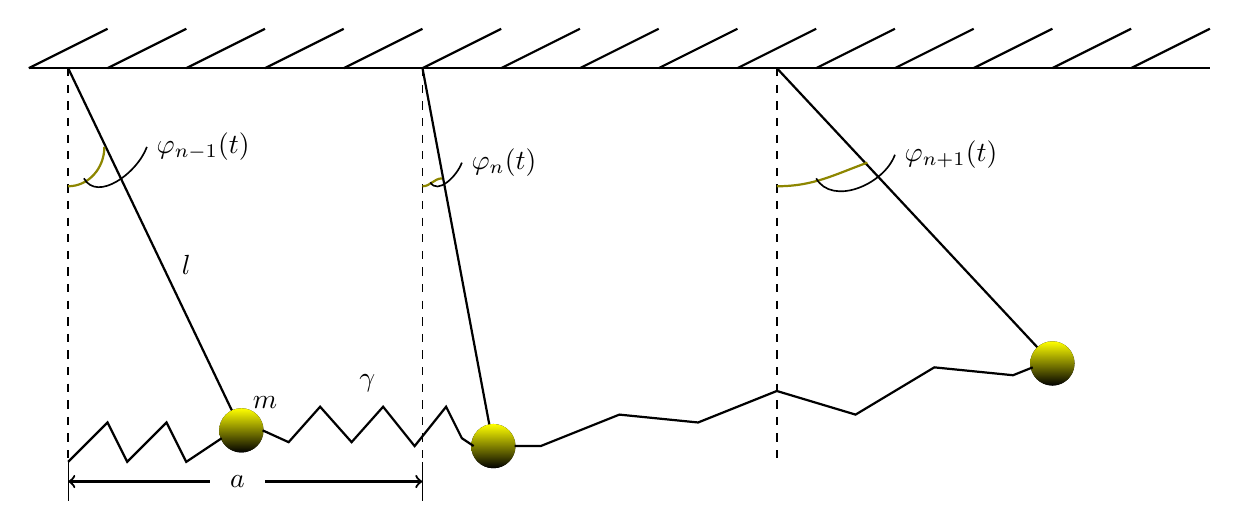
\begin{tikzpicture}
    %пунктирные оси
    \draw [black, dashed, semithick] (1,5.5) -- (1,0.5);
    \draw [black, dashed, semithick] (5.5,5.5) -- (5.5,0.5);
    \draw [black, dashed, semithick] (10,5.5) -- (10,0.5);
    %линия подвеса
    \draw [black, thick] (0.5,5.5) -- (15.5,5.5);
    %верхняя штриховка
    \draw [black, thick] (0.5,5.5) -- (1.5,6);
    \draw [black, thick] (1.5,5.5) -- (2.5,6);
    \draw [black, thick] (2.5,5.5) -- (3.5,6);
    \draw [black, thick] (3.5,5.5) -- (4.5,6);
    \draw [black, thick] (4.5,5.5) -- (5.5,6);
    \draw [black, thick] (5.5,5.5) -- (6.5,6);
    \draw [black, thick] (6.5,5.5) -- (7.5,6);
    \draw [black, thick] (7.5,5.5) -- (8.5,6);
    \draw [black, thick] (8.5,5.5) -- (9.5,6);
    \draw [black, thick] (9.5,5.5) -- (10.5,6);
    \draw [black, thick] (10.5,5.5) -- (11.5,6);
    \draw [black, thick] (11.5,5.5) -- (12.5,6);
    \draw [black, thick] (12.5,5.5) -- (13.5,6);
    \draw [black, thick] (13.5,5.5) -- (14.5,6);
    \draw [black, thick] (14.5,5.5) -- (15.5,6);
    %нити
    \draw [black, thick] (1,5.5) -- (3.2,0.9);
    \draw [black, thick] (5.5,5.5) -- (6.4,0.7);
    \draw [black, thick] (10,5.5) -- (13.5,1.75);
    %шарики
    \shade[top color=yellow, bottom color=black] (3.2,0.9) circle (8pt) [fill=black!];
    \shade[top color=yellow, bottom color=black] (6.4,0.7) circle (8pt) [fill=black!];
    \shade[top color=yellow, bottom color=black] (13.5,1.75) circle (8pt) [fill=black!];
    %пружины
    \draw [black, thick] (1,0.5) -- (1.5,1) --(1.75,0.5) -- (2.25, 1) -- (2.5, 0.5) -- (2.95, 0.8);
    \draw [black, thick] (3.47, 0.9) -- (3.8,0.75) -- (4.2,1.2) -- (4.6, 0.75) -- (5,1.2) -- (5.4, 0.7) --(5.8, 1.2) --(6, 0.8) -- (6.15,0.7); 
    \draw [black, thick] (6.67,0.7) --(7,0.7) -- (8,1.1)--(9,1)--(10,1.4)--(11,1.1)--(12,1.7)--(13,1.6) --(13.25, 1.7);
    %углы
    \draw[olive, thick] (1,4) to [out=0,in=-90] (1.46,4.5);
    \draw[black, semithick] (1.2,4.1) to [out=-60,in=-110] (2,4.5);
    \coordinate [label=right:$\varphi_{n-1}(t)$] (n-1) at (2,4.5);

    \draw[olive, thick] (5.5,4) to [out=0,in=-180] (5.75,4.1);
    \draw[black, semithick] (5.6,4.05) to [out=-60,in=-110] (6,4.3);
    \coordinate [label=right:$\varphi_n(t)$] (n) at (6,4.3);
    
    \draw[olive, thick] (10,4) to [out=0,in=-160] (11.15,4.3);
    \draw[black, semithick] (10.5, 4.1) to [out=-60,in=-110] (11.5, 4.4);
    \coordinate [label=right:$\varphi_{n+1}(t)$] (n+1) at (11.5, 4.4);
    %обозначения 
    \draw [black, thin] (1,0.5) -- (1, 0);
    \draw [black, thin] (5.5,0.5) -- (5.5, 0);
    \draw [black, thick] [->] (2.8, 0.25) -- (1,0.25);
    \draw [black, thick] [->] (3.5, 0.25) -- (5.5,0.25);
    \coordinate [label=center:$a$] (a) at (3.15, 0.25);
    \coordinate [label=center:$m$] (m) at (3.5, 1.25);
    \coordinate [label=center:$\gamma$] (g) at (4.8, 1.5);
    \coordinate [label=center:$l$] (l) at (2.5, 3);
\end{tikzpicture}


\end{document}
